\chapter{Topological states in self-similar lattices}
\label{ch:fractals}
Underlying geometry in quantum lattice models plays an important role in their electronic properties. For instance, frustration in spin models on triangular or kagome lattices arises due to inability of defining unique ground state which minimizes the total energy.


 Having a 

Interestingly, the authors in pointed out that topological states can be realized in amorphous lattice models~\cite{AmorphTIShenoy2017}. BHZ on fractals~\cite{2018:BHZ}






Experimental realizations: CO molecules on a Cu (111) surface \cite{Kempkes2019}, assembled molecules~\cite{Shang2015}, focused ion beam epitaxy~\cite{FIBSC}, in metamaterials that mimic the physics of quantum models (amorphous Chern insulators~\cite{Gyrosc2018Irvine}).



Prediction of peculiar transport properties: \cite{2016:TomadinTransport1, 2017:YuanOptCond}


\section{Real-space methods for computing topological invariants}
Disordered or amorphous systems, due to lack of translational invariance, require defining topological invariants in a real space. Non-commutative
\subsection*{Bott index}
Algorithm for computing the Bott index~\cite{BottIdx}

\subsection*{Chern number}


\begin{equation}
\mathcal{C} = 12 \pi i \sum_{j \in A} \sum_{k \in B} \sum_{l \in C} \left( P_{jk} P_{kl} P_{lj} - P_{jl} P_{lk} P_{kj} \right),
\label{eq: chern_real}
\end{equation}
where $P$ is the projector operator onto occupied states and $i, j, l$ label the lattice sites.

Fractal lattices comprise of many interesting features: they are aperiodic, but scale invariant. Also, there is no sharp notion between bulk and edge.

Here, we are interested in the lattice regularization of two fractals, Sierpiński carpet (SC) and triangle (or gasket) (SG). This approach is relevant for potential experimental realization as it introduces the distance between nearest-neighbouring sites (lattice constant) to be a natural cutoff.

The reason why we investigate these lattices is motivated by their distinct Hausdorff dimensions ($d_H = \ln A / \ln L$, where $A$ is the area and $L$ the linear size) and connectivity properties. Firstly, $d_H = 1.892 \ldots$ for SC and $d_H = 1.585 \ldots$ for SG. 



We consider tight-binding model of spinless electrons exposed to a magnetic field. The Hamiltonian reads
\begin{equation}
H = -t  \sum_{\langle i, j \rangle} e^{\textnormal{i} A_{ij}} c^{\dagger}_i c_j + \mathrm{h.c.},
\label{eq:frac_ham}
\end{equation}
where we set $t = 1$. Introducing a finite field leads to lifting the macroscopic degeneracy

\begin{figure}
\centering
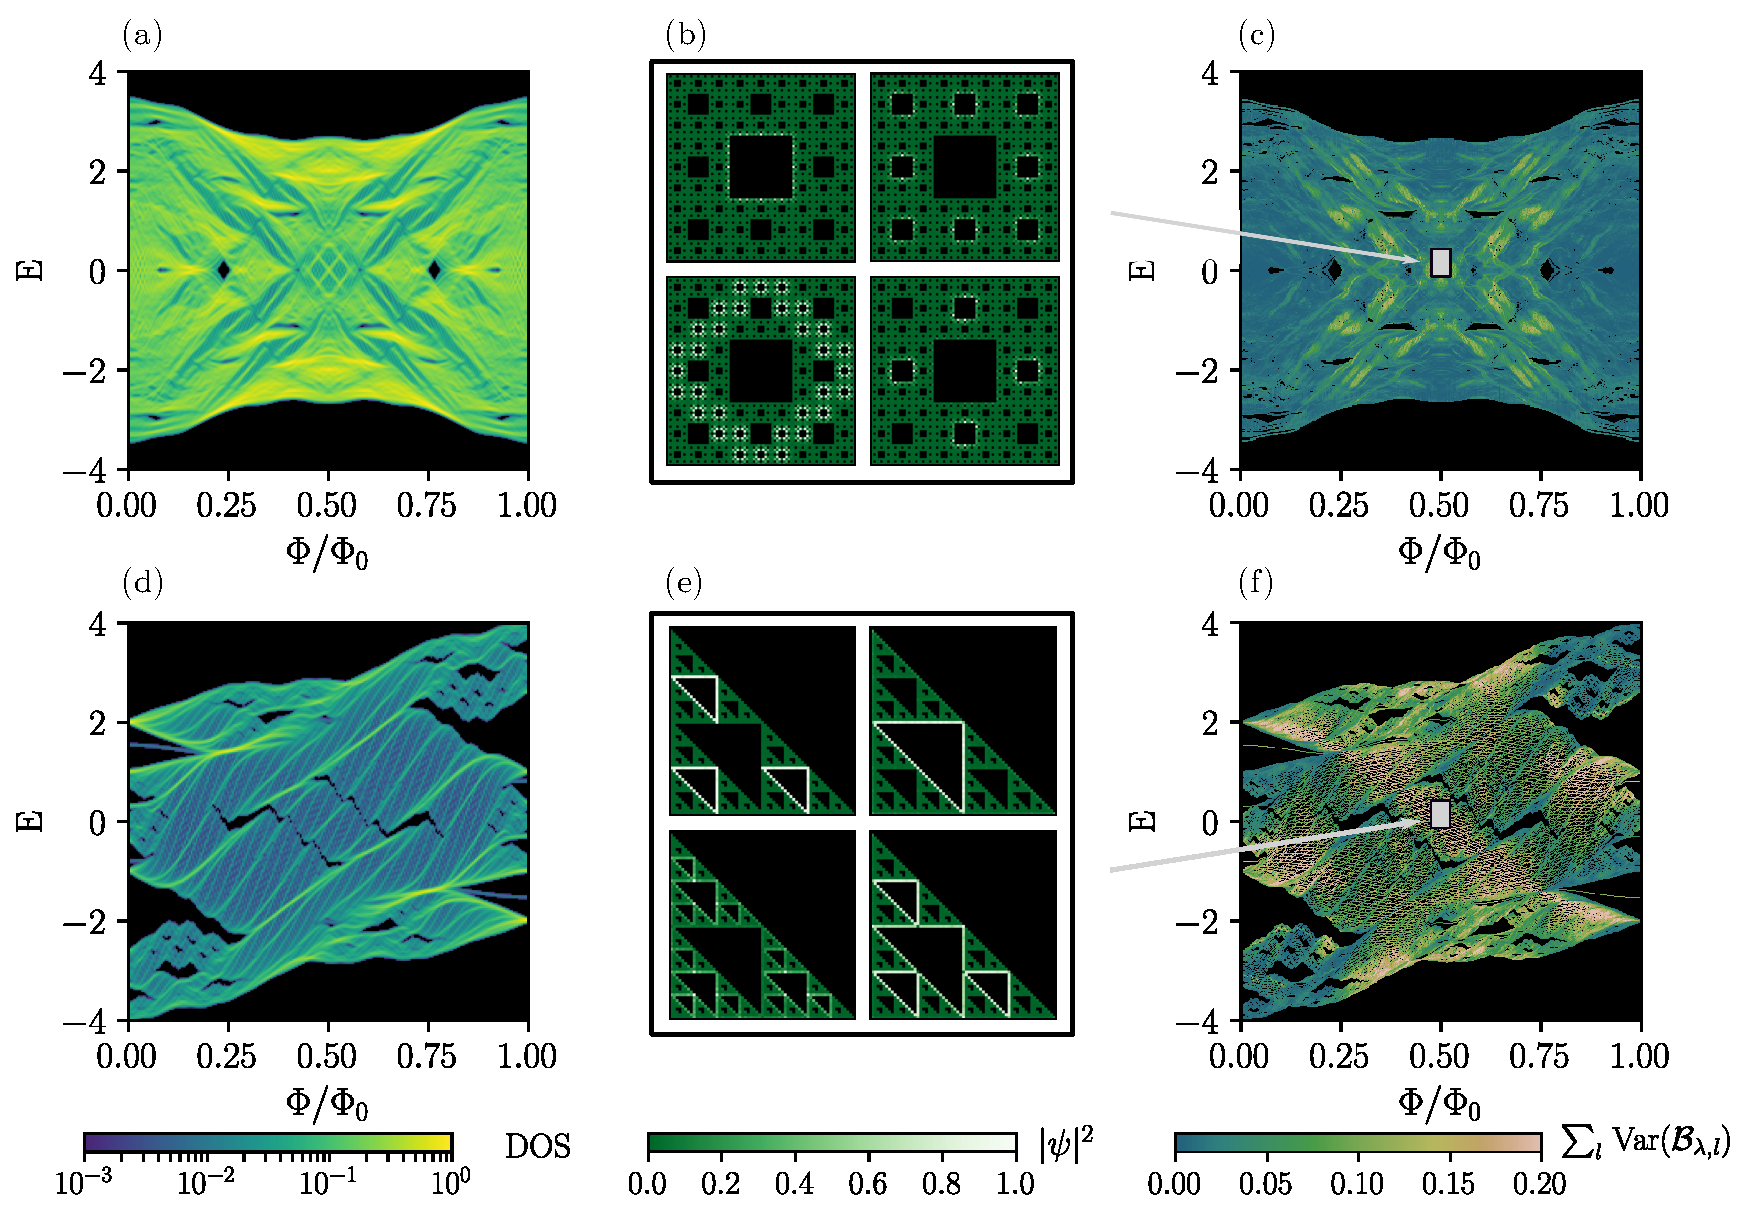
\includegraphics[width=\textwidth]{frac_spectra.eps} 
\caption{Density of states, localization of selected eigenstates and edge-locality marker.}
\label{fig:frac_spect}
\end{figure}

In Fig.~\ref{fig:frac_spect} we observe Hofstadter's butterfly~\cite{1976:Hofstadter}

\begin{figure}
\centering
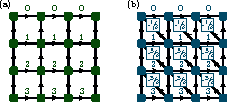
\includegraphics[width=0.5\textwidth]{frac_flux.pdf} 
\caption{Phase distribution on $4 \times 4$ (a) square and (b) triangle lattices with open boundary conditions. $A_{ij}$ phase between site $i$ and $j$ is equal to the number shown above the bond in $2 \pi$ units. A phase acquired with the respect to the direction pointed by arrows has a positive sign.}
\label{fig:flux_distr}
\end{figure}


One of the difficulties is to compute topological invariants in that systems as they do not exhibit translational invariance. One may therefore employ real-space methods. Other methods (for example, the Bott index) may be numerically insufficient. Here, we used the real-space expression for the Chern number:





\begin{figure}
\centering
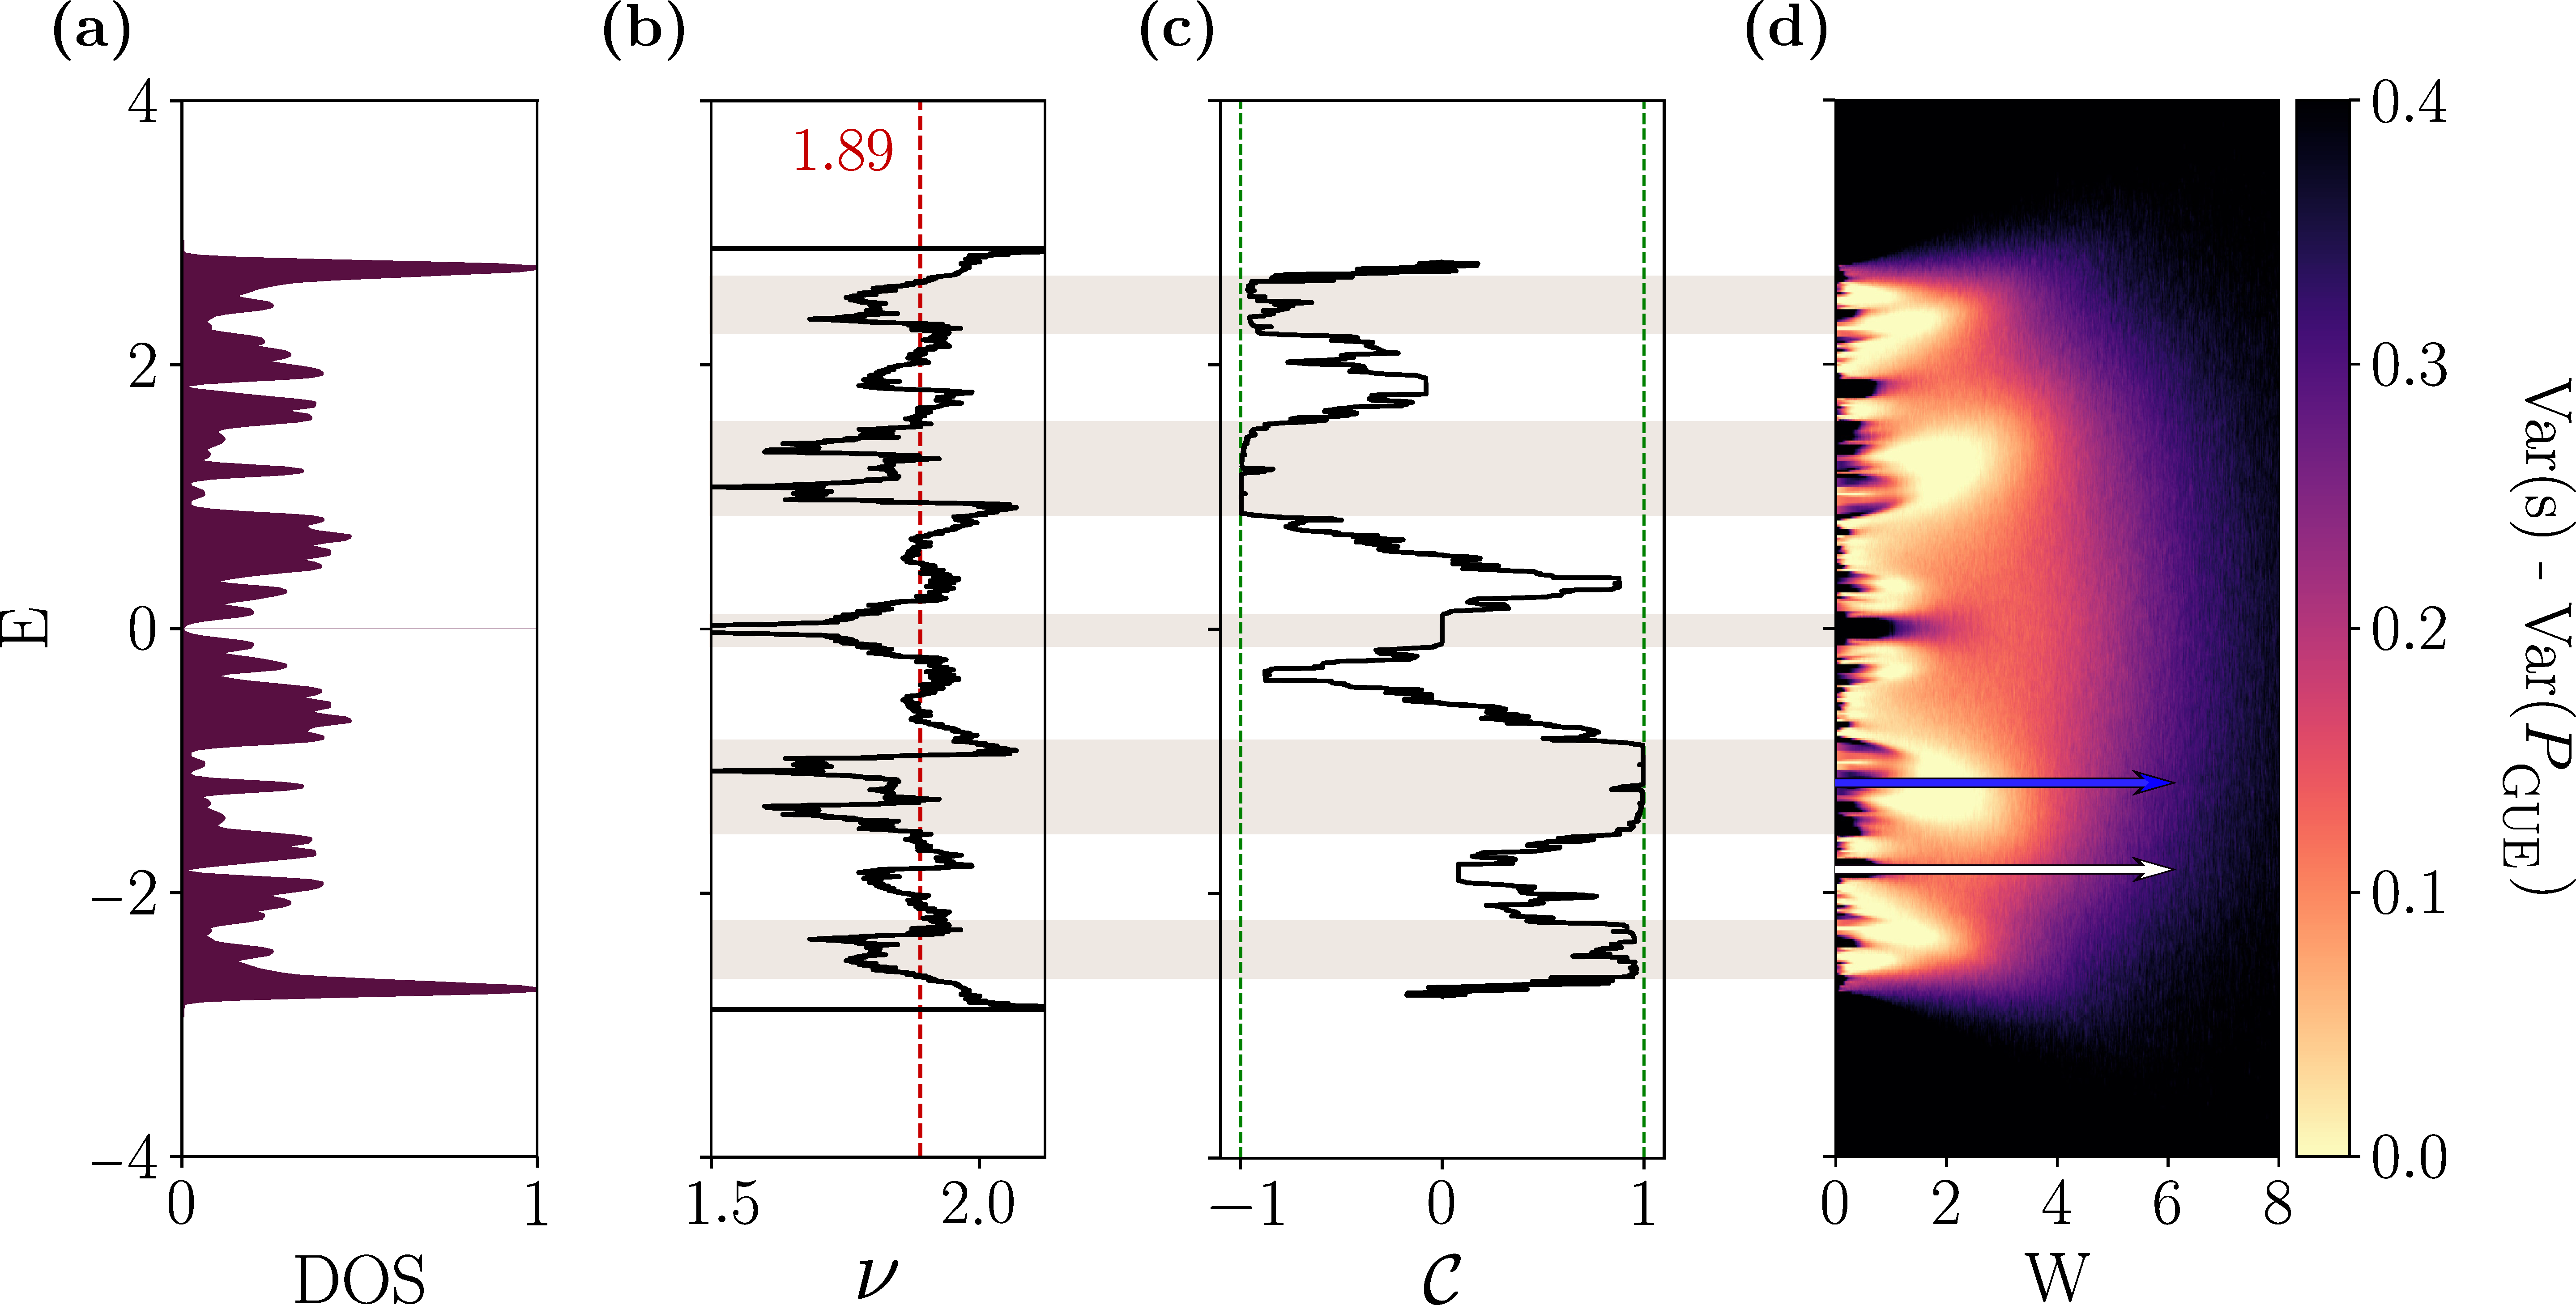
\includegraphics[width=0.5\textwidth]{frac_SC.pdf} 
\caption{Density of states at $\Phi / \Phi_0 = 1/4$, scaling of density of states, the Chern number and disorder-induced phase transition.}
\label{fig:flux_distr}
\end{figure}

To compute the Chern numer as a function of the Fermi level, we use the formula Eq.~\eqref{eq: chern_real}.


\section{Edge states}

Edge-locality marker:

\begin{equation}
\mathcal{B}_{\lambda, l} = \sum_{i \in \mathcal{E}_l} | \psi_{\lambda,i} |^2, 
\label{eq:edgemarker}
\end{equation}
Previous studies for fractal lattices \cite{supp1, supp2} suggested that the presence of a magnetic field leads to an increase in the degree of delocalization of eigenstates. This can be confirmed by calculating inverse participation ratio:
\begin{equation}
I_{\psi} = \frac{\sum_i | \psi_i |^4}{\left(\sum_i  |\psi_i |^2 \right)^2}.
\label{eq:ipr}
\end{equation}

\begin{figure}[h]
\centering
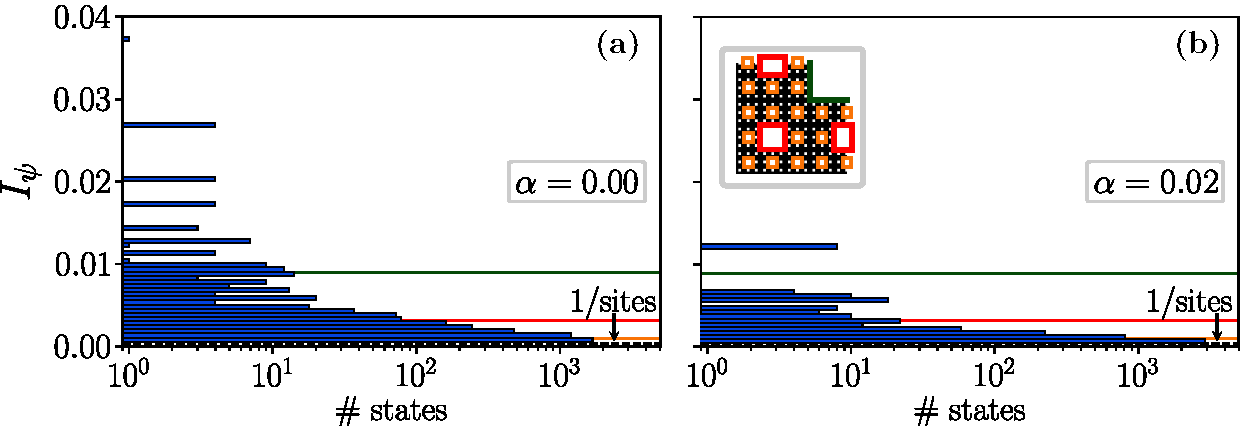
\includegraphics[width = 0.8\columnwidth]{frac_iprSC.pdf}
\caption{Distribution of IPR for SC at (a) $\alpha = 0$ and (b) $\alpha = 0.02$. Inset: a closeup of carpet with internal edges of different hierarchies indicated by distinct colors.}
\label{fig:IPR_SC}
\end{figure}
At zero flux $\alpha = 0$, i.e., in absence of a magnetic field, the distribution of IPRs is peaked close to the inverse of the number of sites belonging to the edges of the second-smallest squares or triangles. As magnetic field is introduced, exemplified here with $\alpha = 0.02$, the distribution of IPRs shifts to smaller, i.e., more delocalized values. This effect is more pronounced for the SC compared to the SG.

\begin{figure}[h]
\centering
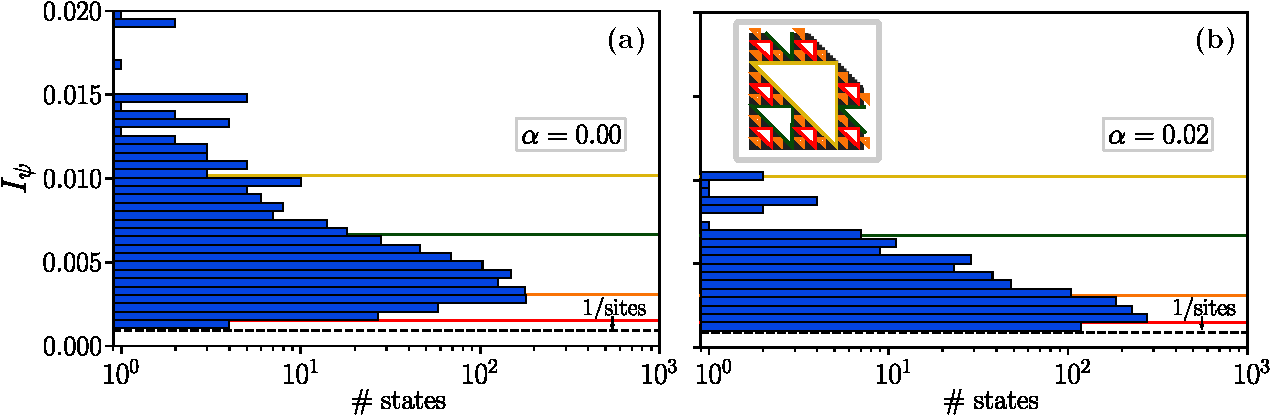
\includegraphics[width = 0.8\columnwidth]{frac_iprSG.pdf}
\caption{Statistics of IPR for SG at (a) $\alpha = 0$ and (b) $\alpha = 0.02$. Inset: a closeup of gasket with highlighted edges of different hierarchies.}
\label{fig:IPR_SG}
\end{figure}


\section{Effect of disorder}

As an ultimate probe, we study potential topological phase transition with the level spacing statistics. Depending whether states are extended or localized, they follow Wigner-Dyson or Poisson distribution, respectively. Such approach was successfully applied to disordered topological and Chern insulators~\cite{2010:ProdanDisordCI, 2011:Prodan}


However, authors in Ref.~\cite{KatnelsonLevels2019} claim that a power-law like level statistics is a generic feature of fractals.

\begin{figure}
\centering
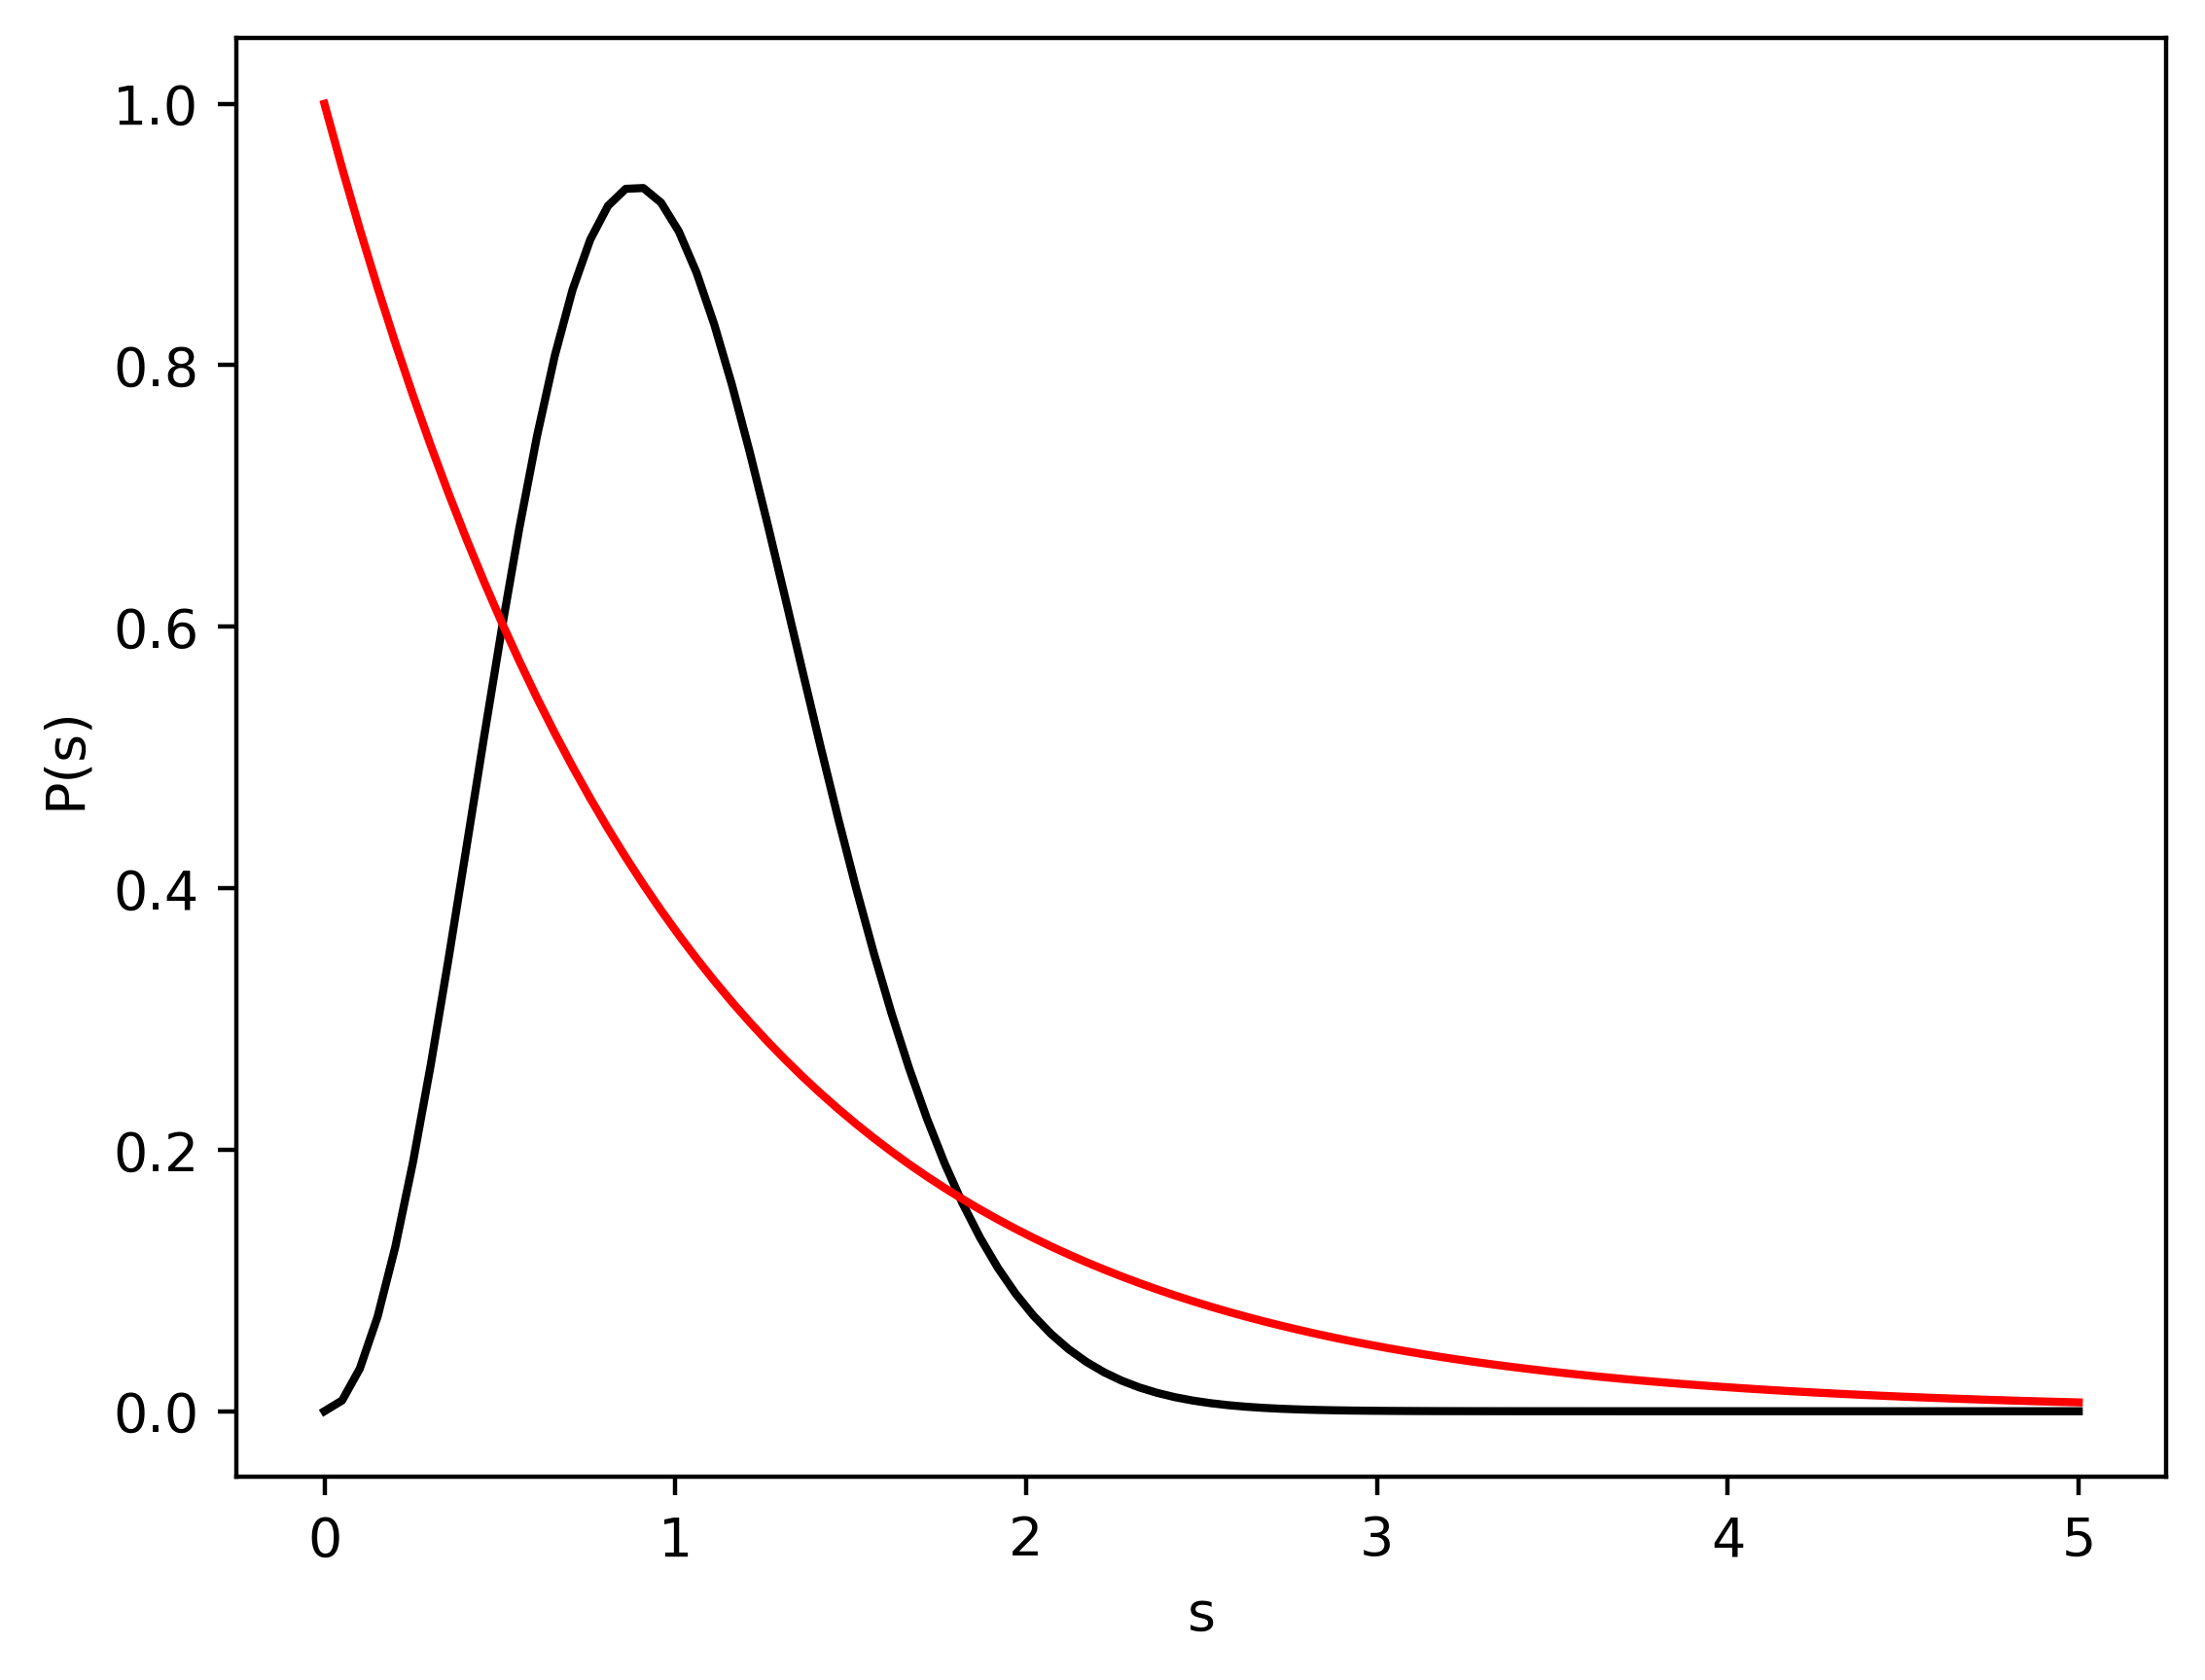
\includegraphics[width=0.5\textwidth]{wd_p_dist.png} 
\caption{Comparison of the level spacing distribution}
\label{fig:ls_distr}
\end{figure}


To do so, we add the on-site disorder term $\sum_i V_i c_i^{\dagger} c_i$ in Eq.~\eqref{eq:frac_ham}, where $V_i$ is drawn from a uniform distribution $[-W/2, W/2 ]$. Having computed the level spacings, we calculate their variance and average over $500$ disorder realizations for each disorder strength $W$.



It is worth mention that follow-up works investigated the Hall conductance in Sierpiński carpet. It was found that the edge states corresponding to non-zero $\sigma_{xy}$ are always present for a finite field strength and stable as one approaches the thermodynamic limit~\cite{EdgesFremling2020}. Interestingly, the Hall conductivity is not proportional to the Chern number~\ctie{KatnelsonFractal2020}. Models realizing spinless chiral $p-$ and $p +ip-$wave superconductors on SC and SG were discussed in~\cite{PaiFractal2019}

